As the behaviour of each individual agent has been described and tested, the next step is looking at a market consisting of some or all of the agents. This has been described in both Oesch 2014 \cite{Oesch} and McG \cite{McGroarty} papers. By comparing the results produced, one can confirm that the agents have been correctly implemented. 

\section{Oesch's Experiment}
\subsection{Oesch's Experiment configuration compared to McG}
McG claims that they have taken the Liquidity consumer and Market maker (Liquidity provider) from the Oesch paper. In addition, both papers referred to Wei and Barbazon \cite{CuiNoise} in Noise trader algorithm. Oesch provides an example result of running the three agents in the same market in addition to the mid price and return series graph. This is a great benchmark to compare whether the agents' behaviour is correct. If the results are similar, it can be concluded that at least three out of five agents are acting correctly when McG results are compared. 

Oesch has a different time step compared to the McG action-step. In each Oesch time-step, a group randomly and uniformly selected between Noise trader, Market maker and Liquidity consumer. Then an agent is selected randomly from the group. The probability of each agent being selected is as follow : 

\begin{table}[h]
\centering
\begin{tabular}{ |m||p{4cm}|} 
\hline
\textbf{Probability of each trader being selected}& \textbf{Value} \\
\hline
\hline
Market maker & 0.15 \\ 
\hline
Liquidity consumer & 0.05\\ 
\hline
Noise Trader & 0.8 \\ 
\hline
\end{tabular}
\caption{Momentum trader parameters taken from \cite{McGroarty}} 
\end{table}
\FloatBarrier 

Unlike McG, when an agent is chosen, it is required to act. The agent can either submit or cancel an order. An order submitted can either be limit order or market order. Other minor changes to the agent are as follow: 

\begin{itemize}
  \item \textbf{Liquidity consumer} : Instead of drawing only from a single large order, if the initial large order at the start of the day is empty, the agent will generate a new one and continue submitting market orders. 
  \item \textbf{Noise Trader} : parameter $xmin_{offspr}$ is 0.05 instead of 0.005. This means that the offspread price generated by the agent will have a higher range then the McG noise agent. 
\end{itemize}

\begin{figure}[h]
  \begin{subfigure}[b]{0.5\textwidth}
    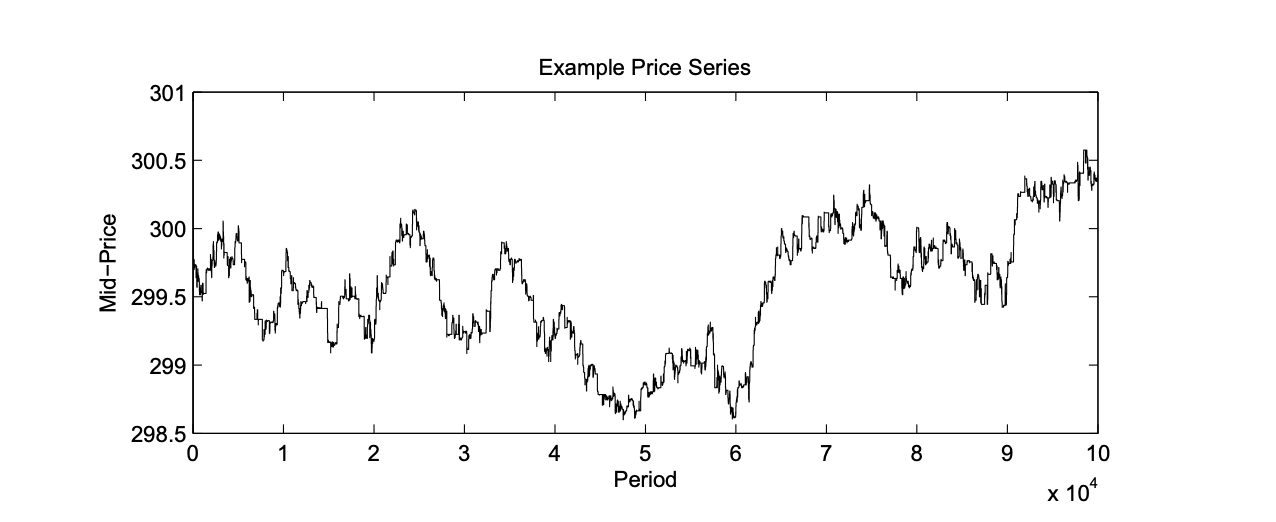
\includegraphics[width=8cm, height=7cm]{Dissertation/images/Market_experiment/Original_mp.png}
    \caption{Mid Price}
    \label{fig:1}
  \end{subfigure}
  %
  \begin{subfigure}[b]{0.5\textwidth}
    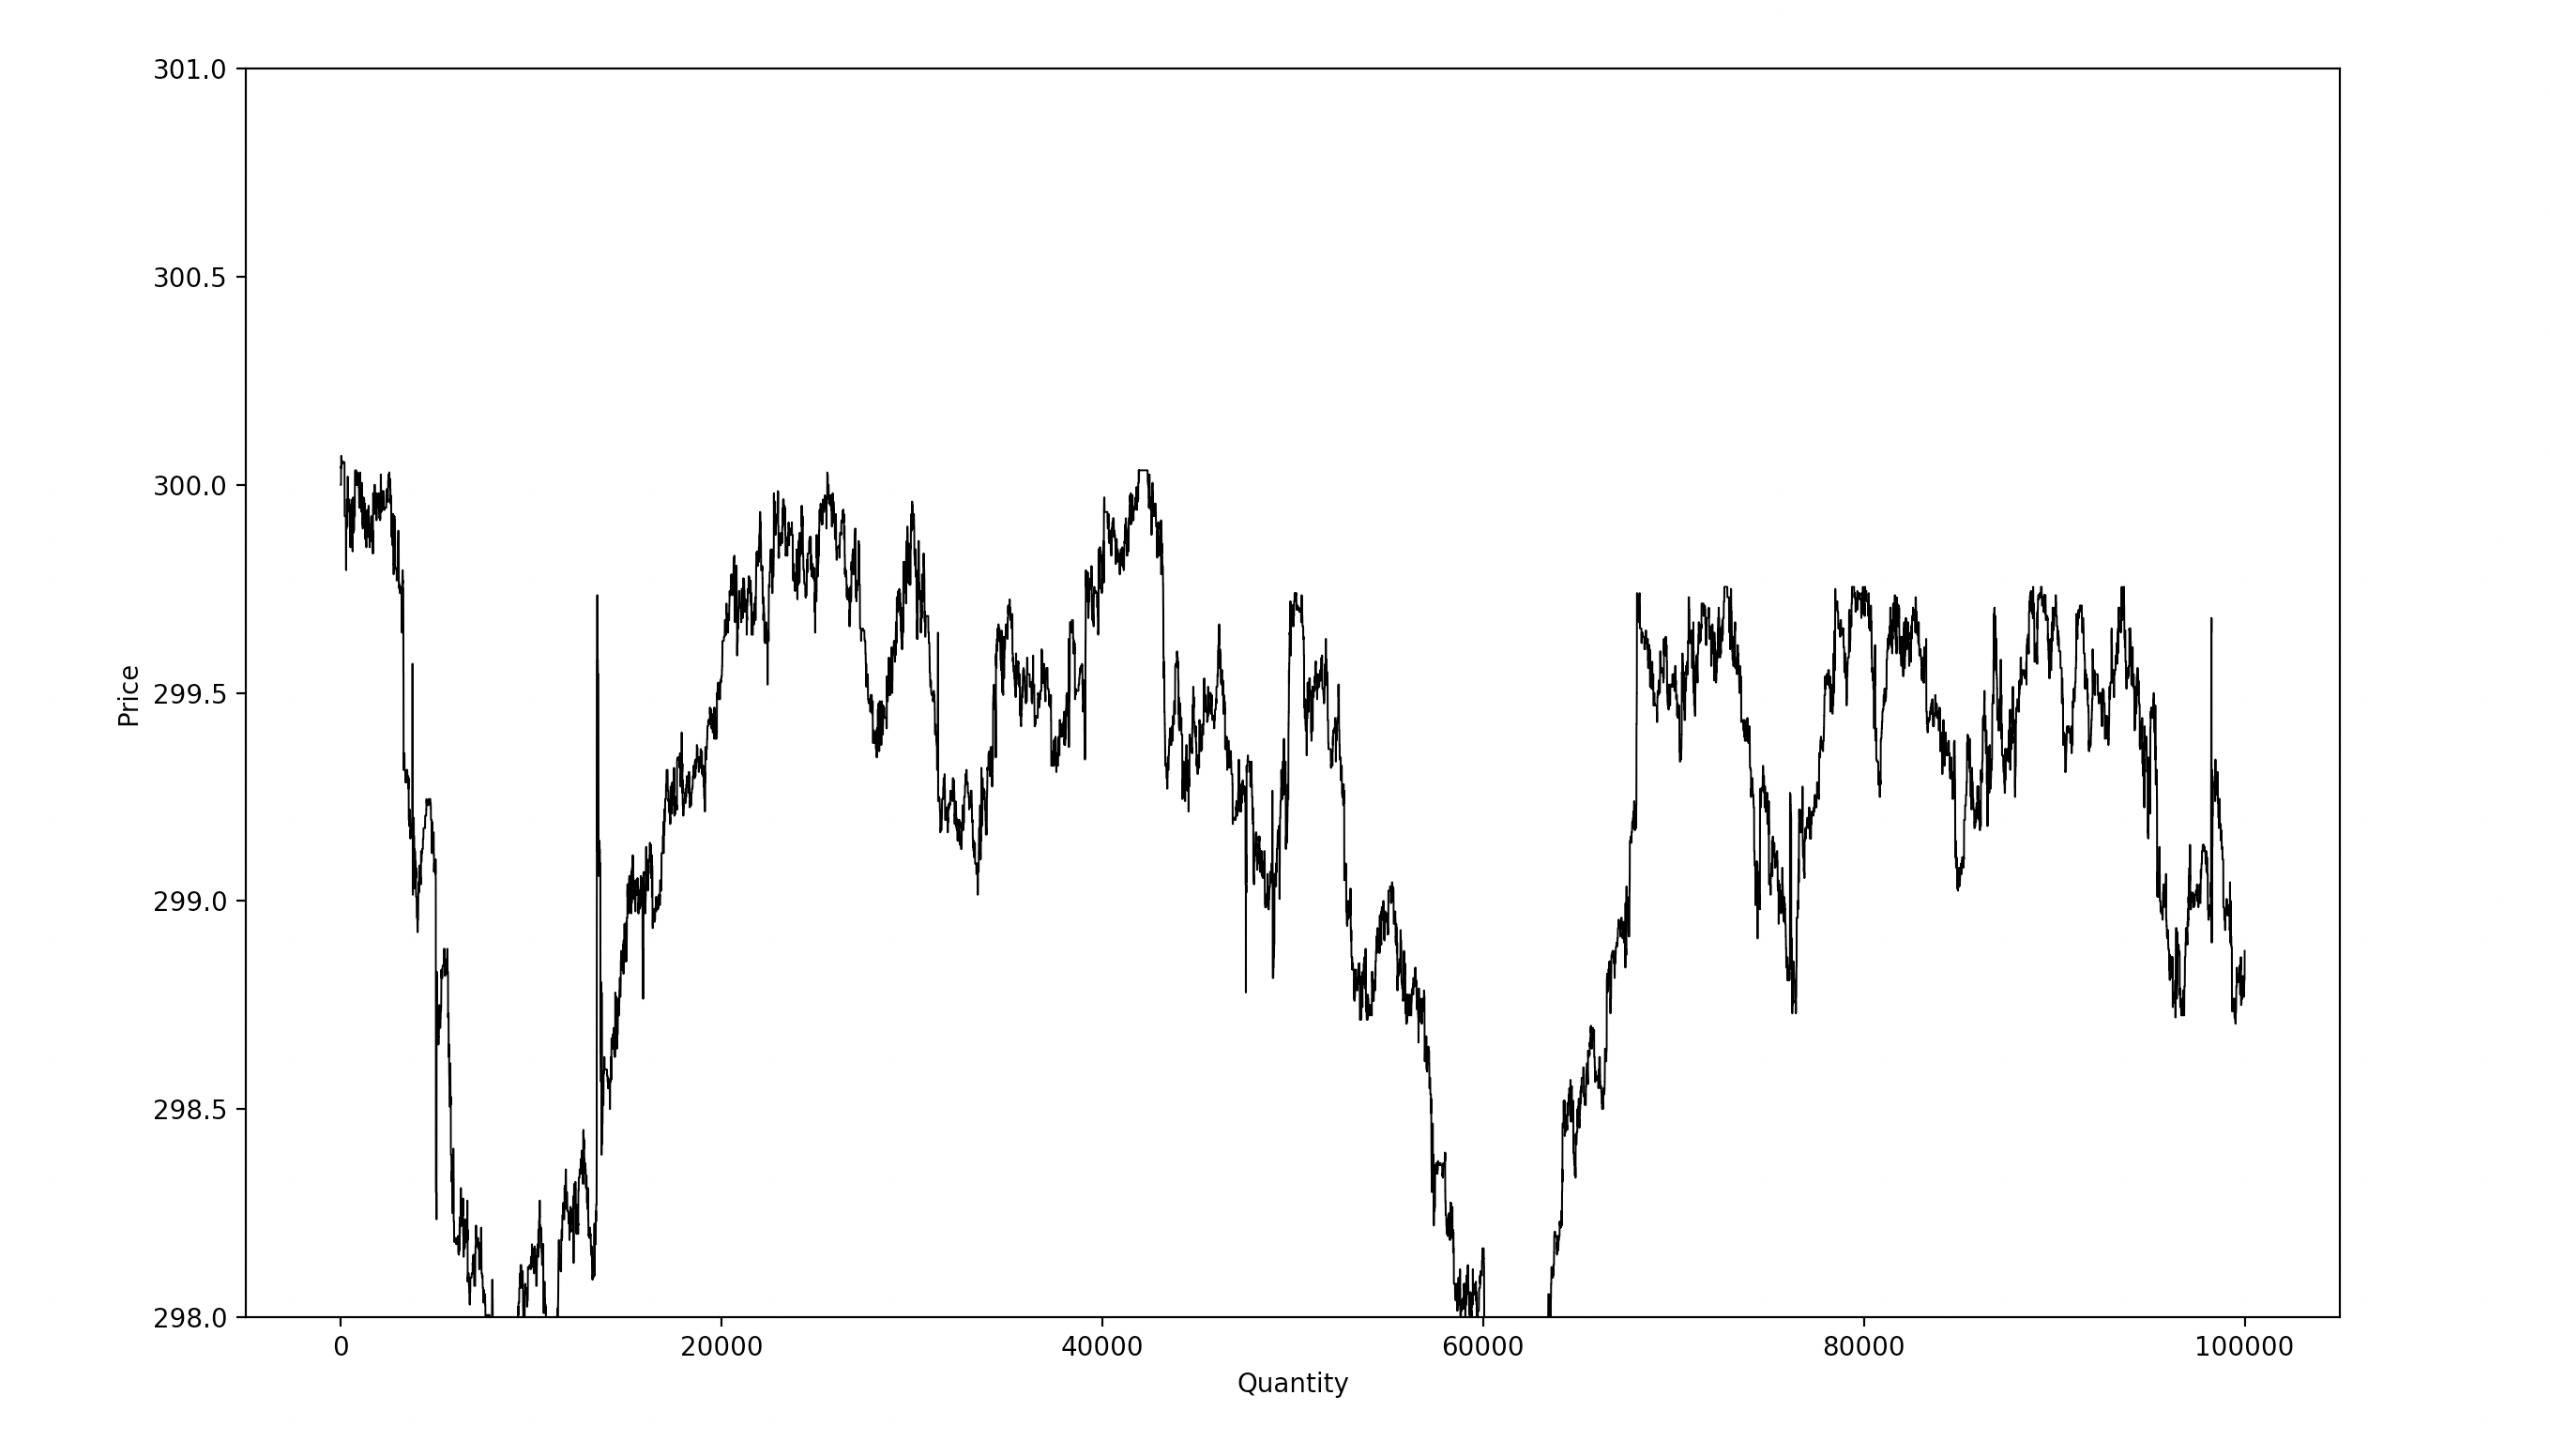
\includegraphics[width= 7cm, height=6cm]{Dissertation/images/Market_experiment/sample2_mp.png}
    \caption{Example Return Series (1 - y values)}
    \label{fig:2}
  \end{subfigure}
\caption{Replication of Oesch's experiments with similar configurations} 
\end{figure}

\begin{figure}[h]
  \begin{subfigure}[b]{0.5\textwidth}
    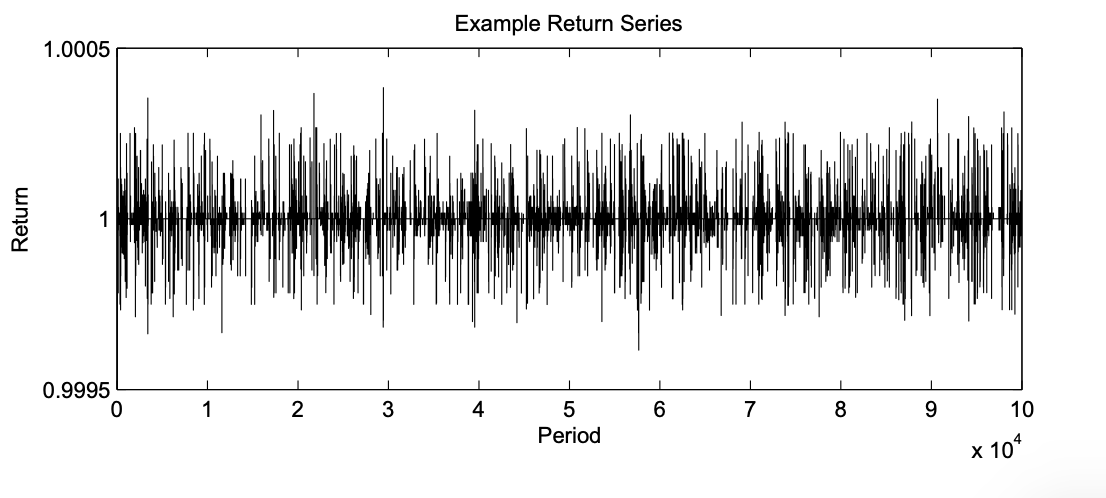
\includegraphics[width=7cm, height=6cm]{Dissertation/images/Market_experiment/Original_return.png}
    \caption{Mid Price}
    \label{fig:1}
  \end{subfigure}
  %
  \begin{subfigure}[b]{0.5\textwidth}
    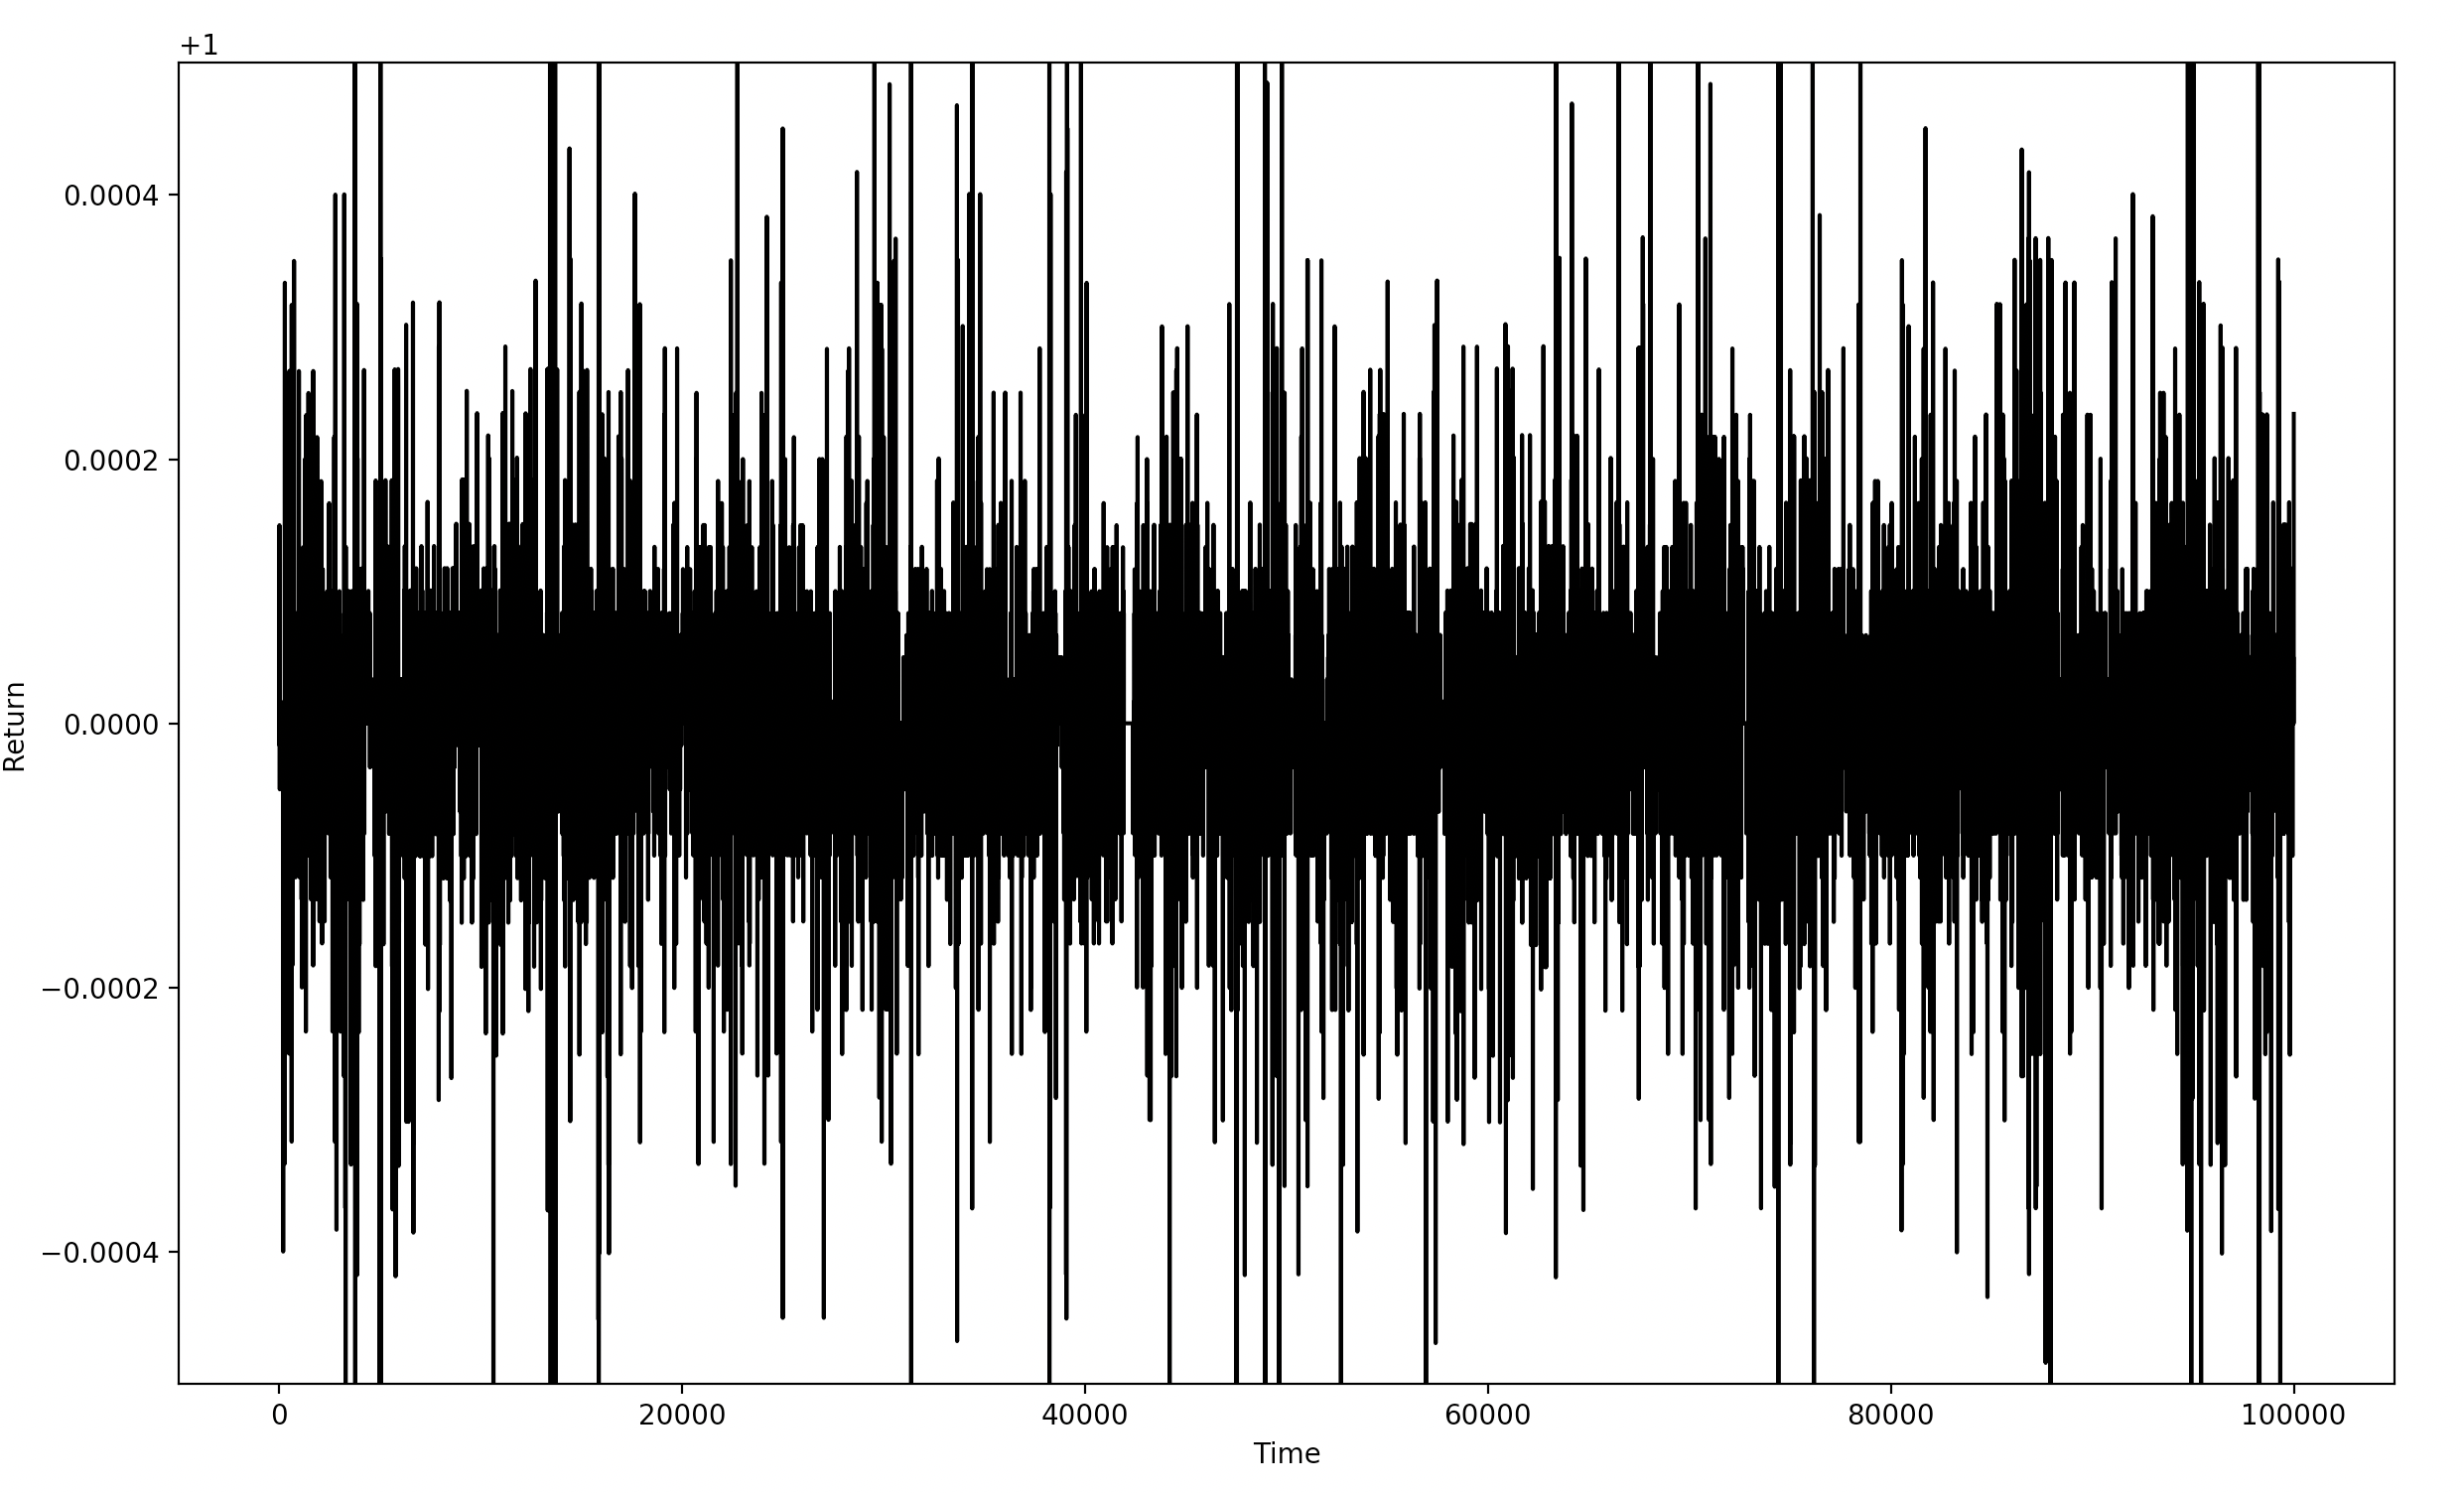
\includegraphics[width= 7cm, height=6cm]{Dissertation/images/Market_experiment/sample2_return.png}
    \caption{Example Return Series (1 - y values)}
    \label{fig:2}
  \end{subfigure}
\caption{Replication of Oesch's experiments with similar configurations} 
\end{figure}

Figure 6.2 depicts the results after replication of Oesch's experiment. The market consists of 40 of each trader. The mid price value is still in range of the original experiment, which is between 298.5 and 301. The price movement exhibits similar movements over the period of time. There are some important factors that contribute to why the results may not be totally similar. 

\begin{itemize}
  \item Oesch's results in mid price and return series does not state how many or what is the ratio of the agent types in the market when the experiment is being conducted.
  \item The details of the agents are all explained verbally, which may not be as detailed as the one described in McG with clear algorithm. There are obvious difference between the agents in the two papers and the difference in results can be correlated with the missing details of the agents in Oesch's. 
\end{itemize}